%!TEX root = dissertation.tex
\chapter{Introduction}
\label{chap:intro}
In signal processing, statistics, and machine learning, it is common to consider that noisy measurements/data are generated from a latent, unknown, function. In statistics, this is often regarded as a regression problem over the space of functions. Specifically, Bayesian statistics impose a prior belief over the latent function of interest in the form of a probability distribution. It is therefore of vital importance to choose the prior appropriately, since it will encode the characteristics of the underlying function. In recent decades, Gaussian processes\footnote{In the statistics and applied probability literature, Gaussian processes can also be found under the name of Gaussian fields, in particular when they are multidimensional in the input. Depending on the context, we may use one or the other terminology interchangeably.}~\citep[GPs,][]{Carl2006GPML} have become a popular family of prior distributions over functions, and they have been used successfully in numerous applications~\citep{Roberts2013, Hennig2015, Kocijan2016}.

Formally, GPs are function-valued random variables that have Gaussian distributions fully determined by their mean and covariance functions. The choice of mean and covariance functions is in itself arbitrary, which allows for representing functions with various properties. As an example, \matern covariance functions are used as priors to functions with different degrees of differentiability~\citep{Carl2006GPML}. However, the use of GPs in practice usually involves two main challenges.

The first challenge lies in the expensive \textit{computational cost} of training and parameter estimation. Due to the necessity of inverting covariance matrices during the learning phase, the computational complexity of standard GP regression and parameter estimation is cubic in the number of measurements. This makes GP computationally infeasible for large-scale datasets. Moreover, when the sampled data points are densely located, the covariance matrices that need inversion may happen to be numerically singular or close to singular, making the learning process unstable.

The second challenge is related to modelling of irregular functions, such as piecewise smooth functions, or functions that have time-varying features (e.g., frequency or volatility). Many commonly-used GPs (e.g., with \matern covariance functions) fail to cover these irregular functions mainly because their probability distributions are invariant under translation (i.e., they are said to be \textit{stationary}). This behaviour is illustrated in Figure~\ref{fig:gp-fail}, where we show that a \matern GP poorly fits two irregular functions (i.e., a rectangular signal and a composite sinusoidal signal), because the GP's parameters/features are assumed to be constant over time. Specifically, in the rectangular signal example, in order to model the discontinuities, the \matern GP recovers a small global length scale ($\ell \approx 0.04$) which results in poor fitting in the continuous and flat parts. Similarly, in the composite sinusoidal signal example, the GP learns a small global length scale ($\ell \approx 0.01$) in order to model the high-frequency sections of the signal. This too results in poor fitting the low-frequency section of the signal.

\begin{figure}[t!]
	\centering
	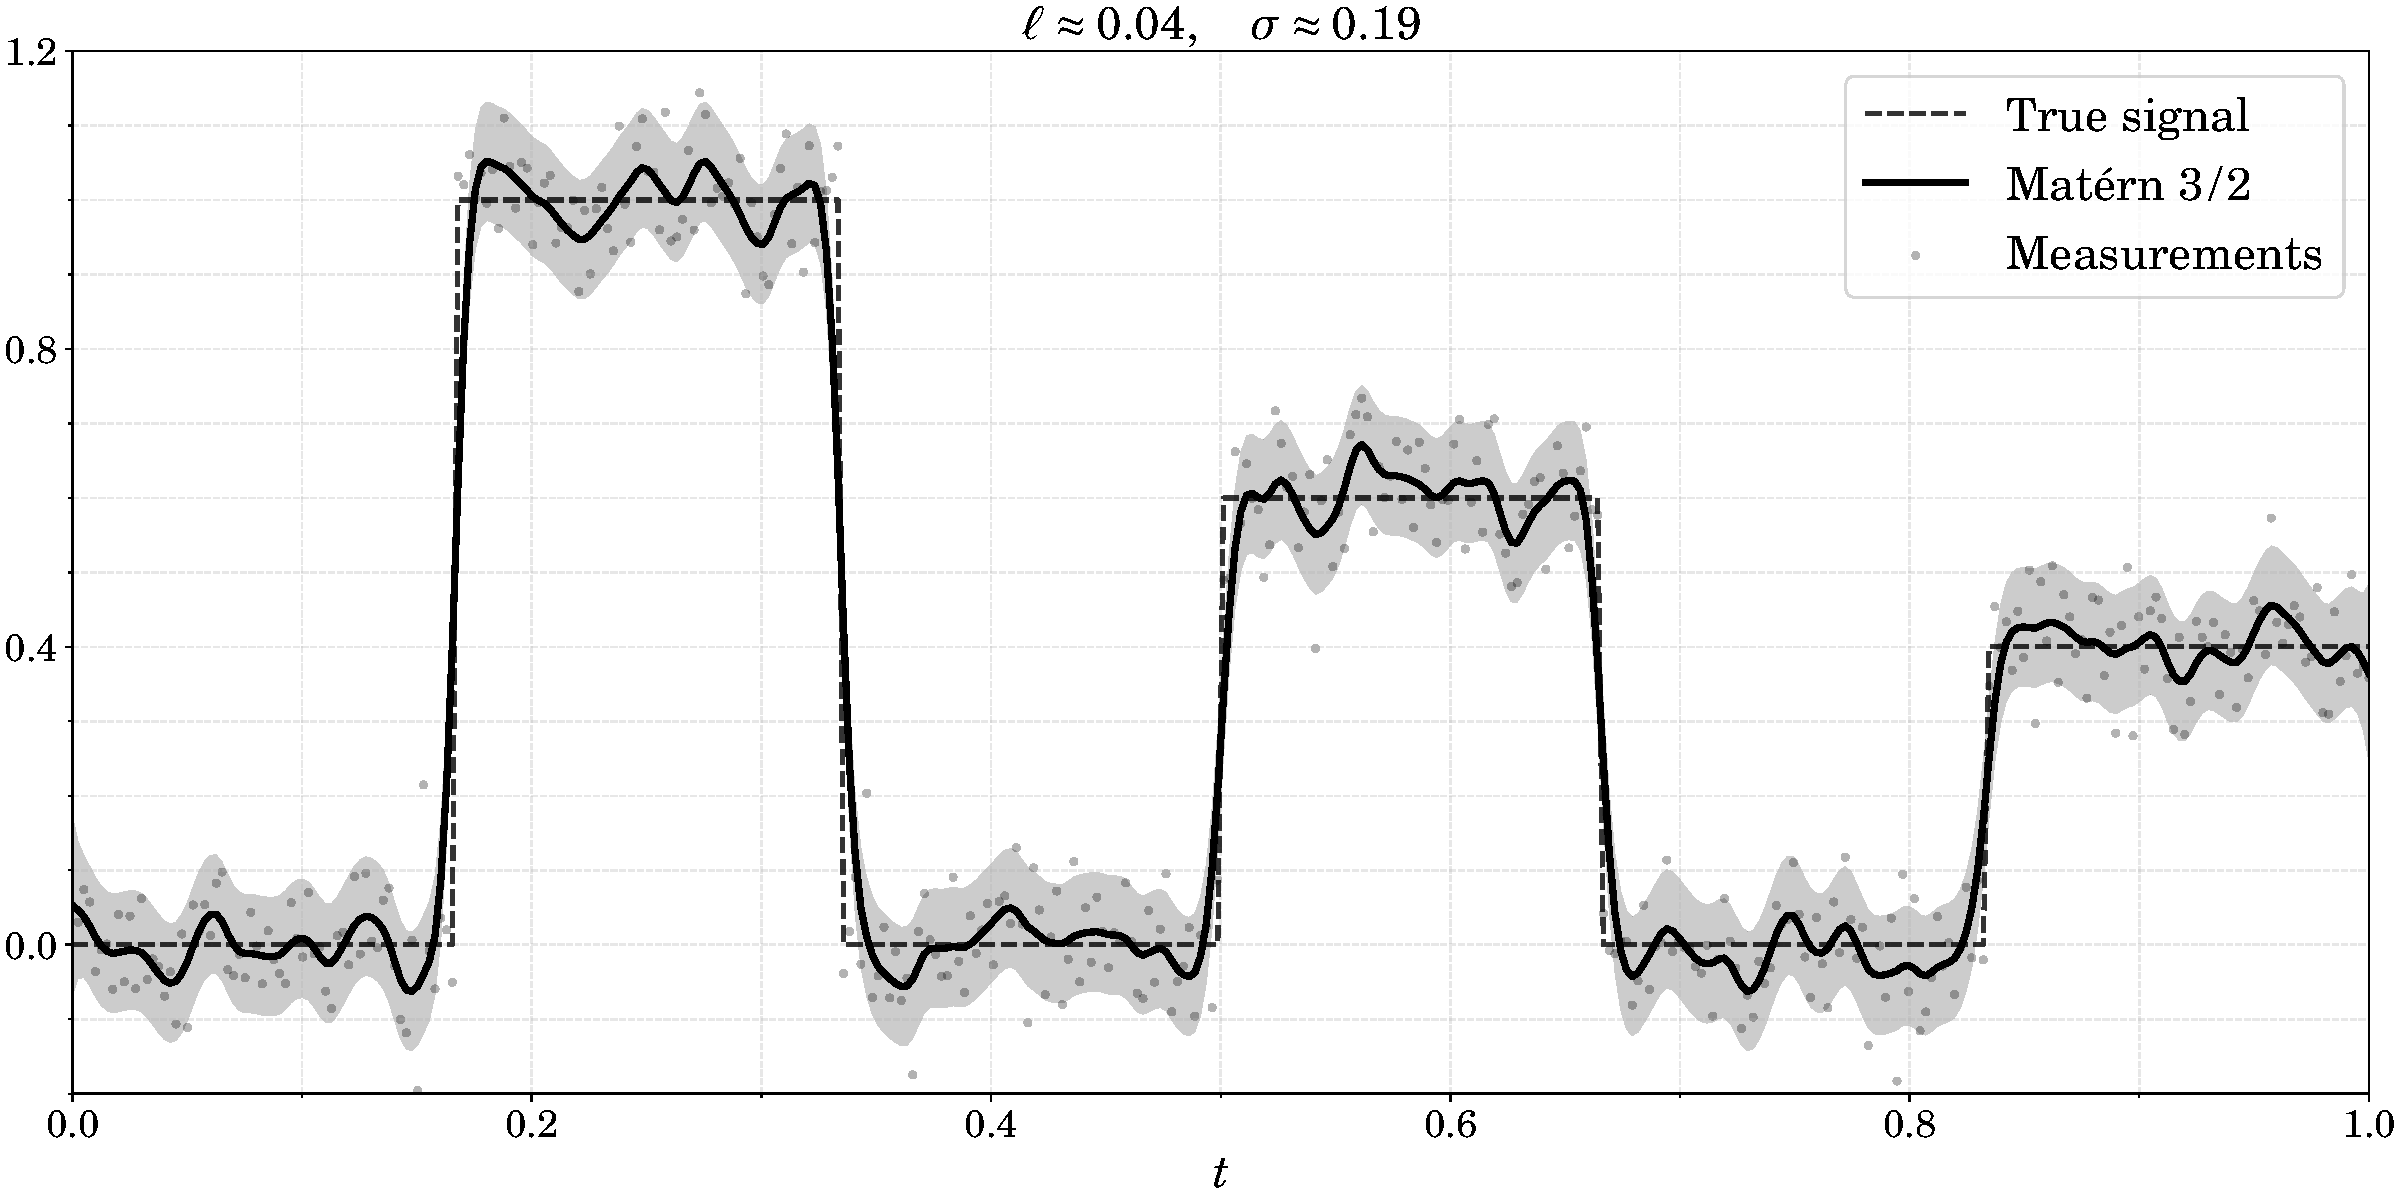
\includegraphics[width=.95\linewidth]{figs/gp-fail-example-m32}\\
	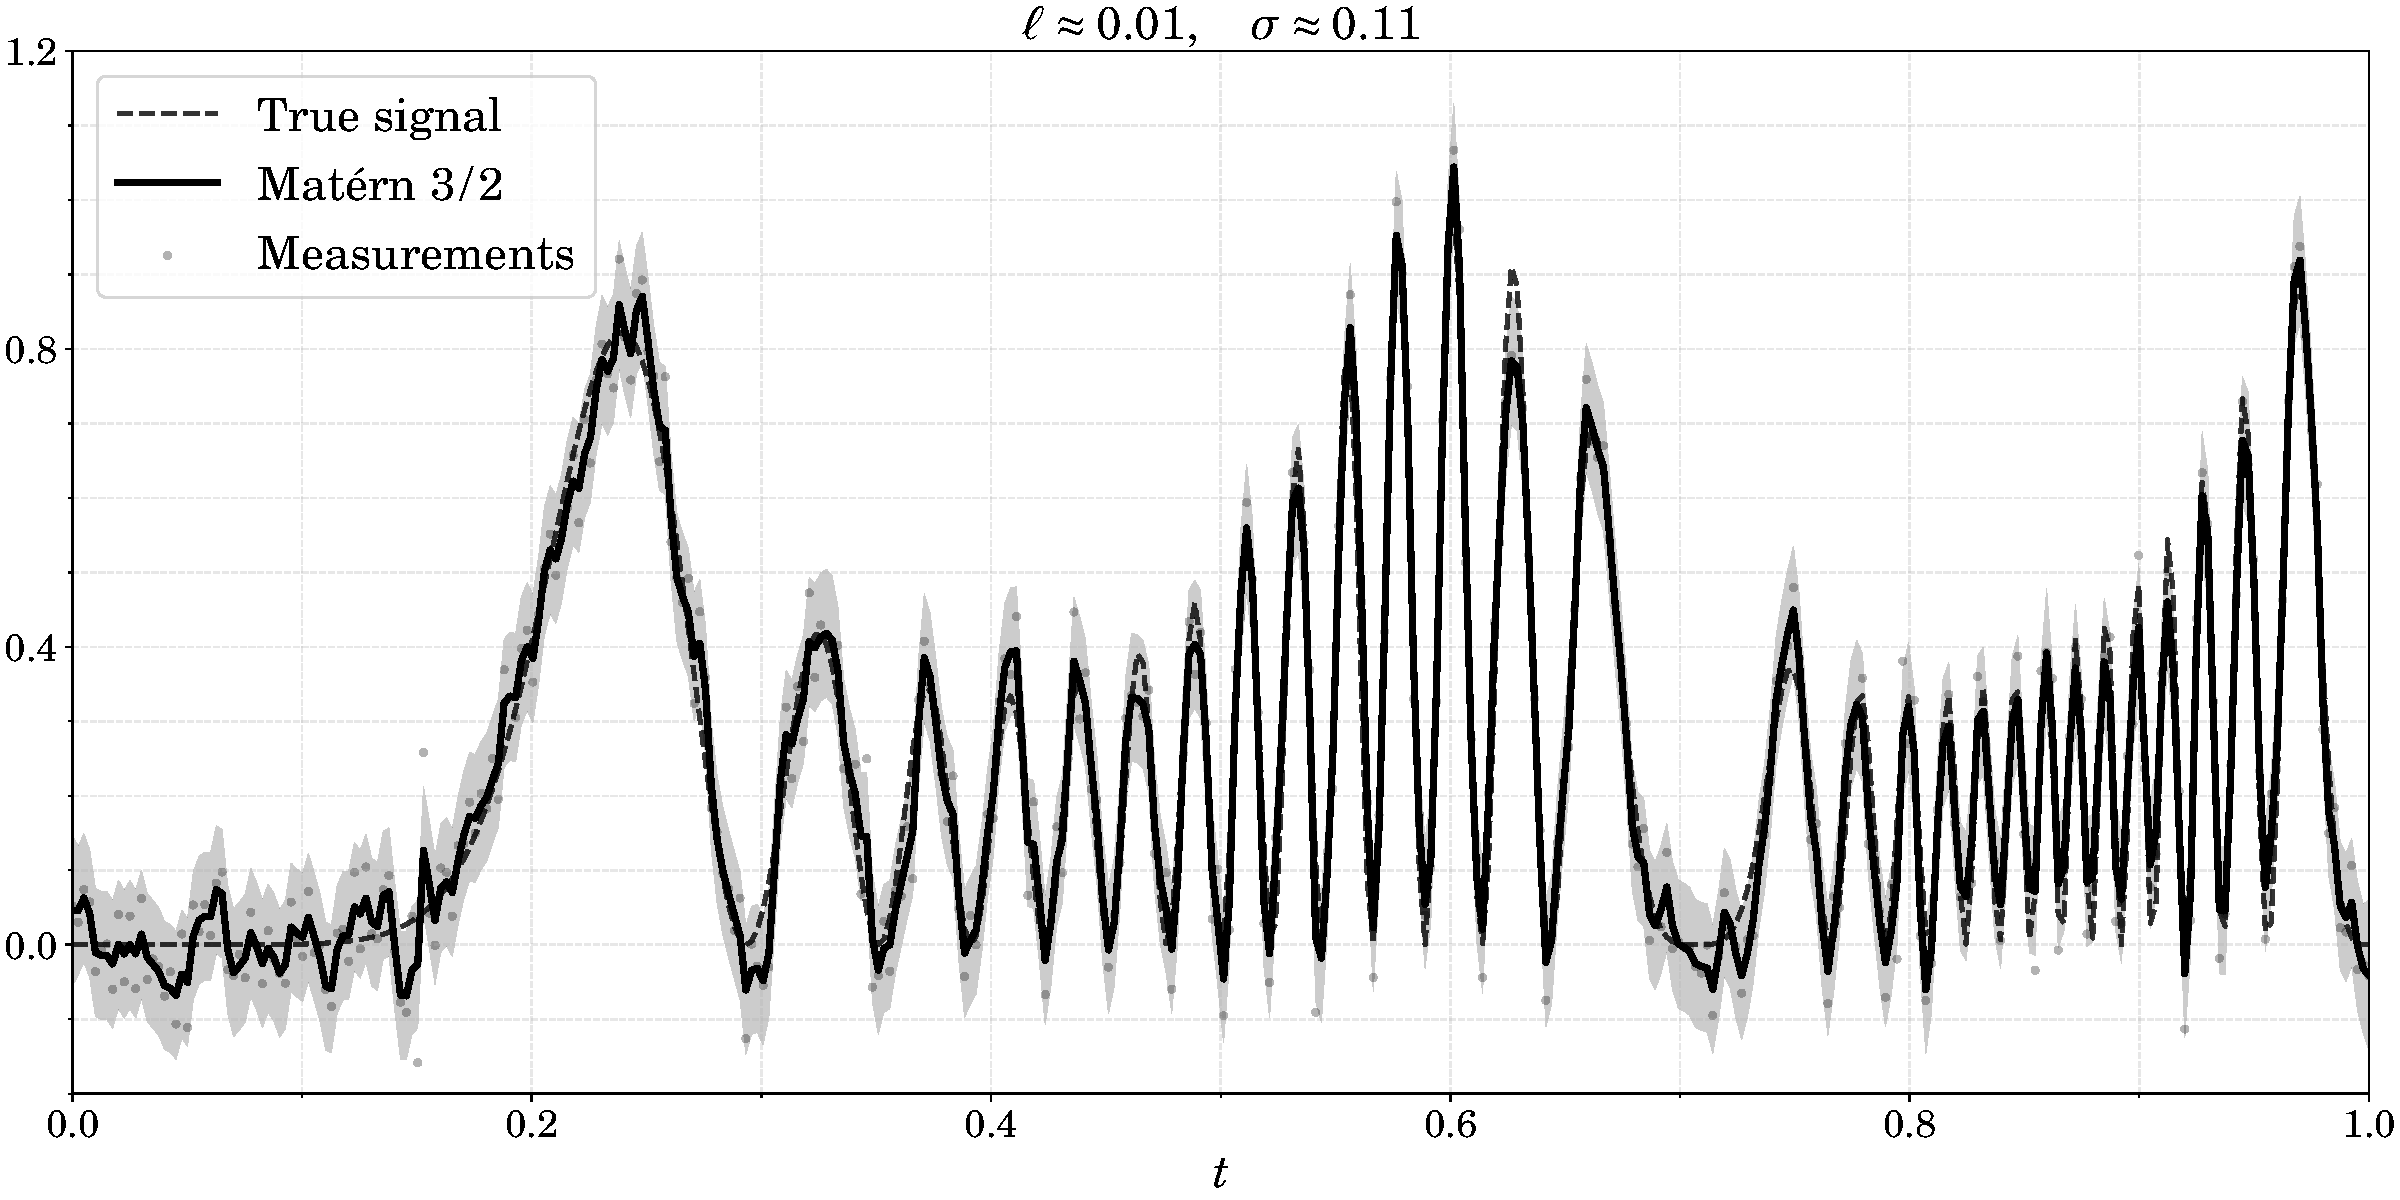
\includegraphics[width=.95\linewidth]{figs/gp-fail-example-sinu-m32}
	\caption{Mat\'{e}rn $\nu=3\,/\,2$ GP regression on a magnitude-varying rectangular signal (top) and a composite sinusoidal signal (bottom). The parameters $\ell$ and $\sigma$ are learnt by maximum likelihood estimation. The figures are taken from~\citet{Zhao2020SSDGP}.}
	\label{fig:gp-fail}
\end{figure}

The main aim of this thesis is thus to introduce a new class of non-stationary (Gaussian) Markov processes, that we name \textit{state-space deep Gaussian processes (SS-DGPs)}\footnote{Please note that although the name includes the term Gaussian, SS-DGPs are typically not Gaussian distributed, but instead hierarchically conditionally Gaussian, hence the name.}. These are able to address the computational and non-stationarity challenges aforementioned, by hierarchically composing the state-space representations of GPs. Indeed, SS-DGPs are computationally efficient models due to their Markovian structure. More precisely, this means that the resulting regression problem can be solved in linear computational time (with respect to the number of measurements) by using Bayesian filtering and smoothing methods. Moreover, due to their hierarchical nature, SS-DGPs are capable of changing their features/characteristics (e.g., length scale) over time, thereby inducing a rich class of priors compatible with irregular functions. The thesis ends with a collection of applications of state-space (deep) GPs.

\section{Bibliographical notes}
\label{sec:literature-review}
In this section we provide a short and non-exhaustive review of related works in the GP literature. In particular we will focus on works that consider specifically reducing their computational complexity and allowing the non-stationarity in GPs.

\subsection*{Scalable Gaussian processes}
We now give a list of GP methods and approximations that are commonly used to reduce the computational costs of GP regression and parameter learning.

\subsubsection{Sparse approximations of Gaussian processes}
Sparse GPs approximate full-rank GPs with sparse representations by using, for example, inducing points~\citep{Snelson2006}, subsets of data~\citep{Snelson2007, Csato2002}, or approximations of marginal likelihoods~\citep{Titsias2009}, mostly relying on so-called pseudo-inputs. These approaches can reduce the computational complexity to quadratic in the number of pseudo-inputs and linear in the number of data points. In practice, the number and position of pseudo-inputs used in sparse representation must either be assigned by human experts or learnt from data~\citep{Hensman2013}. For more comprehensive reviews of sparse GPs, see, for example,~\citet{Quinonero2005unifying, Chalupka2013, LiuHaitao2020}.

\subsubsection*{Gaussian Markov random fields}
Gaussian Markov random fields~\citep[GMRFs,][]{Rue2005Book} are indexed collections of Gaussian random variables that have a Markov property (defined on graph). They are computationally efficient models because their precision matrices are sparse by construction. Methodologies for solving the regression and parameter learning problems on GMRFs can be found, for example, in~\citet{Rue2007, Rue2009N}. However, GMRFs are usually only approximations of Gaussian fields~\citep[see, e.g.,][Chapter 5]{Rue2005Book}, although explicit representations exist for some specific Gaussian fields~\citep{Lindgren2011}.

\subsubsection*{State-space representations of Gaussian processes}
State-space Gaussian processes (SS-GPs) are (temporal) Markov GPs that are solutions of stochastic differential equations~\citep[SDEs,][]{Simo2013SSGP, Sarkka2019}. Due to their Markovian structure, probability distributions of SS-GPs factorise sequentially in the time dimension. The regression problem can therefore be solved efficiently in linear time with respect to the number of data points. Moreover, leveraging the sparse structure of the precision matrix \citep{Grigorievskiy2017}, or leveraging the associativity of the Kalman filtering and smoothing operations \citep{Corenflos2021SSGP} can lead to a sublinear computational complexity.

\subsubsection*{Other data-scalable Gaussian processes}
\citet{Rasmussen2002GPexperts, Meeds2006} form mixtures of GPs by splitting the dataset into batches resulting in a computational complexity that is cubic in the batch size. This methodology can further be made parallel \citep{ZhangMinyi2019}. \citet{Lazaro2010} approximate stationary GPs with sparse spectral representations (i.e., trigonometric expansions). \citet{Gardner2018} and \citet{KeWang2019} use conjugate gradients and stochastic trace estimation to efficiently compute the marginal log-likelihood of standard GPs, as well as their gradients with respect to parameters, resulting in a quadratic computational complexity in the number of data points.

\subsection*{Non-stationary Gaussian processes}
In the below we give a list of methods that are introduced in order to induce non-stationarity in GPs.

\subsubsection*{Non-stationary covariance function-based Gaussian processes}
Non-stationary covariance functions can be constructed by making their parameters (e.g., length scale or magnitude) depend on the data position. For instance, \citet{Gibbs} and \citet{Higdon1999non} present specific examples of covariance functions where the length scale parameter depends on the spatial location. On the other hand, \citet{Paciorek2004, Paciorek2006} generalise these constructions to turn any stationary covariance function into a non-stationary one. There also exist some other non-stationary covariance functions, such as the polynomial or neural network covariance functions~\citep{Williams1998, Carl2006GPML} that can also give non-stationary GPs, but we do not review them here as they are not within the scope of this thesis. 

\subsubsection*{Composition-based Gaussian processes}
\citet{Sampson1992, Schmidt2003, Carl2006GPML} show that it is possible to construct a non-stationary GP as the pullback of an existing stationary GP by a non-linear transformation. Formally, given a stationary GP $U\colon E \to \R$, one can find a suitable transformation $\Upsilon\colon \T \to E$, such that the composition $U \circ \Upsilon\colon \T\to\R$ is a non-stationary GP on $\T$. For example, \citet{Calandra2016ManifoldGP} and~\citet{Wilson2016DeepKernel} choose $\Upsilon$ as neural networks.

\subsubsection{Warping-based Gaussian processes}
Conversely to the composition paradigm above, it is also possible to transform GPs the other way around, that is, to consider that GPs are the transformations of some non-Gaussian processes by non-linear functions~\citep{Snelson2004}. Computing the marginal log-likelihood function of these warped GPs is then done by leveraging the change-of-variables formula for Lebesgue integrals (when it applies). However, the warping can be computationally demanding as the change-of-variables formula requires computing the inverse determinant of the transformation Jacobian. This issue can be mitigated, for example, by writing the the warping scheme with multiple layers of elementary functions which have explicit inverses~\citep{Rios2019}.


\subsection*{Deep Gaussian processes}
The deterministic constructions for introducing non-stationarity GPs can be further extended in order to give a class of non-stationary non-Gaussian processes that can also represent irregular functions. While they are different in structure, the three subclasses of models presented below are usually all referred as deep Gaussian processes (DGPs) in literature.

\subsubsection*{Composition-based deep Gaussian processes}
\citet{Gredilla2012} extends the aforementioned pullback idea by taking $\Upsilon\colon \T\to E$ to be a GP instead of a deterministic mapping in order to overcome the overfitting problem. Resulting compositions of the form $U \circ \Upsilon\colon \T\to\R$ may not necessarily be GPs anymore but may provide a more flexible family of priors than that of deterministic compositions. This construction can be done recursively leading to a subclass of DGPs~\citep{Damianou2013}. However, the training of these DGPs is found to be challenging and requires approximate inference methods~\citep{Bui2016, Salimbeni2017Doubly}. Moreover, \citet{Duvenaud2014Thesis, Duvenaud2014} show that increasing the depth of DGPs can lead to a representation pathology, where samples of DGPs tend to be flat in high probability and exhibit sudden jumps. This problem can be mitigated by making their latent GP components explicitly depend on their original inputs~\citep{Duvenaud2014}.

\subsubsection*{Hierarchical parametrisation-based deep Gaussian processes}
A similar idea to compositional DGPs is to model the parameters of GPs as latent GPs. The posterior distribution of the joint model can then be computed by successive applications of Bayes' rule. As an example,~\citet{Roininen2016} consider putting a GP prior on the length scale parameter of a \matern GP and use Metropolis-within-Gibbs to sample from the posterior distribution. Similarly,~\citet{Salimbeni2017ns} model the length scale parameter of the non-stationary covariance function introduced by~\citet{Paciorek2004} as a GP, but use a variational approximation to approximate its posterior distribution. Other sampling techniques to recover the posterior distribution of these models can be found, for example, in~\citet{Heinonen2016, Karla2020}. 

\citet{Zhao2020SSDGP} and~\citet{Emzir2020} show that this hierarchy in parametrisation can be done recursively, leading to another subclass of DGPs that can be represented by stochastic (partial) differential equations. The relationship between the composition-based and parametrisation-based DGPs is also briefly discussed in~\citet{Dunlop2018JMLR}.

\section{Reproducibility}
\label{sec:codes}
In order to allow for reproducibility of our work, we provide  the following implementations.

\begin{itemize}
	\item Taylor moment expansion (Chapter~\ref{chap:tme}). Python and Matlab codes for it are available at \href{https://github.com/zgbkdlm/tme}{https://github.com/zgbkdlm/tme}.
	\item State-space deep Gaussian processes (Chapter~\ref{chap:dssgp}). Python and Matlab codes for it are available at \href{https://github.com/zgbkdlm/ssdgp}{https://github.com/zgbkdlm/ssdgp}.
	\item The Python codes for reproducing Figures~\ref{fig:gp-fail}, \ref{fig:disc-err-dgp-m12}, \ref{fig:ssdgp-vanishing-cov}, and~\ref{fig:spectro-temporal-demo}, as well as the simulations in Examples~\ref{example-tme-benes}, \ref{example:tme-softplus}, \ref{example:ssdgp-m12}, and~\ref{example:ssdgp-m32} are available at \href{https://github.com/zgbkdlm/dissertation}{https://github.com/zgbkdlm/dissertation}.
\end{itemize}

\section{Outline of the thesis}
\label{sec:outline}
This thesis consists of seven publications and overviews of them, and the thesis is organised as follows.

In Chapter~\ref{chap:cd-smoothing} we review stochastic differential equations (SDEs) and Bayesian continuous-discrete filtering and smoothing (CD-FS) problems. This chapter lays out the preliminary definitions and results that are needed in the rest of the thesis. 

Chapter~\ref{chap:tme} (related to Publication~\cp{paperTME}) shows how to solve Gaussian approximated CD-FS problems by using the Taylor moment expansion (TME) method. This chapter also features some numerical demonstrations and analyses the positive definiteness of TME covariance approximations as well as the stability of TME Gaussian filters.

Chapter~\ref{chap:dssgp} (related to Publications~\cp{paperSSDGP} and~\cp{paperRNSSGP}) introduces SS-DGPs. In particular, after defining DGPs formally, we introduce their state-space representations. Secondly, we present how to sample from SS-DGPs by combining discretisation and numerical integration. Thirdly, we illustrate the construction of SS-DGPs in the \matern sense. Fourhtly, we represent SS-DGP regression problems as CD-FS problems that we can then solve using the methods introduced in Chapter~\ref{chap:cd-smoothing}. Finally, we explain how DGPs can be regularised in the $L^1$ sense, in particular to promote sparsity at any level of the DGP component hierarchy.

Chapter~\ref{chap:apps} (related to Publications~\cp{paperDRIFT},~\cp{paperKFSECG},~\cp{paperKFSECGCONF},~\cp{paperSSDGP}, and~\cp{paperMARITIME}) introduces various applications of state-space (deep) GPs. These include estimation of the drift functions in SDEs, probabilistic spectro-temporal signal analysis, as well as modelling real-world signals (from astrophysics, human motion, and maritime navigation) with SS-DGPs.

Finally, Chapter~\ref{chap:summary} offers a summary of the contributions of the seven publications presented in this thesis, and concludes with a discussion of unsolved problems and possible future extensions. 
